\documentclass[11pt,letterpaper]{article}
\usepackage[lmargin=1in,rmargin=1in,tmargin=1in,bmargin=1in]{geometry}
\usepackage{../style/homework}
\usepackage{../style/commands}
\setbool{quotetype}{false} % True: Side; False: Under
\setbool{hideans}{true} % Student: True; Instructor: False

% -------------------
% Content
% -------------------
\begin{document}

\homework{11: Due 04/14}{The power of mathematics is often to change one thing into another, to change geometry into language.}{Marcus du Sautoy}

% Problem 1
\problem{10} The speed of an airplane is 821.3~ft/s. Find this speed in miles per hour (mph). [Note: 5280~ft $=$ 1~mi]



\newpage



% Problem 2
\problem{10} Find $x$ in the diagram below:
	\[
	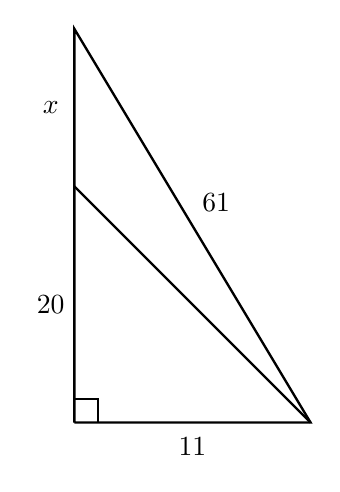
\begin{tikzpicture}
	\draw[line width=0.03cm] (0,0) -- (0,5) -- (3,0) -- (0,0);
	\draw[line width=0.03cm] (0,0.3) -- (0.3,0.3) -- (0.3,0);
	\draw[line width=0.03cm] (3,0) -- (0,3);
	\node at (1.5,-0.3) {$11$};
	\node at (-0.3,1.5) {$20$};
	\node at (1.8,2.8) {$61$};
	\node at (-0.3,4.0) {$x$};
	\end{tikzpicture}
	\]



\newpage



% Problem 3
\problem{10} A `track' consists of two semicircles adjoined to the sides of a rectangle. Find the perimeter and the area of the `track' below.
	\[
	\begin{tikzpicture}
	\draw[line width=0.03cm] (0,0) -- (8,0);
	\draw[line width=0.03cm] (0,4) -- (8,4);
	\draw[line width=0.03cm] (8,4) -- (8,0) arc(-90:90:2);
	\draw[line width=0.03cm] (0,0) -- (0,4) arc(90:270:2);
	\draw[line width=0.04cm,white] (0,0.015) -- (0,3.985);
	\draw[line width=0.03cm,dotted] (0,0.015) -- (0,3.985);
	\draw[line width=0.04cm,white] (8,0.015) -- (8,3.985);
	\draw[line width=0.03cm,dotted] (8,0.015) -- (8,3.985);
	\node at (4,-0.3) {$88$~m};
	\node at (0.6,2) {$46$~m};
	\end{tikzpicture}
	\]


\end{document}